\documentclass[12pt,a4paper]{article}
\usepackage[utf8x]{inputenc}
\usepackage{ucs}
\usepackage[catalan]{babel}
\usepackage{amsmath}
\usepackage{amsfonts}
\usepackage{amssymb}
\usepackage{graphicx}
\usepackage{algpseudocode}
\usepackage{algorithm}
\usepackage{float}
\usepackage{caption}
\usepackage{subcaption}
\usepackage{multirow}
\usepackage{fullpage}
\usepackage[hidelinks]{hyperref}
\usepackage{url}

\DeclareMathOperator*{\argmax}{arg\,max}

\author{Joan Puigcerver i Pérez\\
\begin{footnotesize}joapuipe@upv.es\end{footnotesize}}
\title{Connecta-4: Implementació del joc i una heurística per guanyar-lo}

\begin{document}
\maketitle
\abstract{Aquest article resumeix el projecte fet per a l'assignatura \emph{Aplicació de Tècniques d'Intel·Ligència Artificial} dins del Màster en Intel·ligència Artificial, Reconeixement de Formes i Imatge Digital impartit en la Universitat Politècnica de València. L'objectiu era el de construïr un programa d'ordinador capaç de jugar al joc \emph{Connecta-4} i una heurística capaç de vèncer a un oponent de nivell mitjà, estudiant així les distintes tècniques d'Intel·ligència Artificial per a jocs de suma zero. Durant el transcurs d'aquest projecte s'ha dissenyat també un algorisme genètic per ajustar  els paràmetres d'una de les heurístiques, aplicant també tècniques d'Algorismes Genètics per a obtenir una millor heurística. El codi font del projecte està disponible en \url{https://github.com/jpuigcerver/miarfid-atia-connect4}.}

\section{Introducció}
El \emph{Connecta-4} o \emph{Quatre en línia} és un joc de taula per a dos jugadors aparegut el 1974 de la mà de l'empresa nordamericana Milton Bradley i que ràpidament es popularitzà, convertint-se en un dels jocs de taula més coneguts del món.\\

El joc consisteix en un tauler vertical format per 7 columnes i 6 files, amb un total de 42 cel·les que poden ser ocupades per uns discs que representen a cadascun dels dos jugadors. Cada disc es suporta sobre el fons del tauler o sobre un disc anterior en la mateixa columna. Els jugadors, col·locant un disc en cada torn, han d'omplir el tauler intentant aconseguir que quatre dels seus discs siguen adjacents de manera vertical, horitzontal o seguint alguna de les diagonals del tauler.\\

El primer jugador en formar el grup de quatre discs, guanya la partida. Si el tauler s'ompli completament i cap jugador ha format un grup de quatre discs, llavors empaten. Existeixen altres modalitats de joc, però aquesta és l'original i la més estesa.\\

En 1988, James D. Allen\cite{allen1989note} i Victor Allis\cite{allis1988knowledge} demostraren independentment que, fent els moviments adequats, el jugador que comença el joc pot forçar una victòria, independentment de l'estratègia del segon jugador. El segon ho feu introduint 9 regles que determinaven el moviment a fer per el jugador òptim segons l'estat del tauler i a més demostrà que si el primer jugador no seguia aquestes regles i el segon jugador sí, el segon podia forçar almenys un empat.\\

A pesar de que el joc es considere solucionat, segueix sent molt popular i és un dels clàssics a l'hora d'introduir conceptes d'Intel·ligència Artificial en jocs d'ordinador. A més, les regles creades per Allis sols són òptimes donades certes condicions per al tauler de joc, de manera que encara resulta interessant dissenyar bons programes d'Intel·ligència Artificial que puguen jugar de la millor manera sobre qualsevol tauler.\\

Aquest treball pretèn implementar el joc \emph{Connecta-4} per ordinador i una Intel·ligència Artificial el millor possible (almenys, capaç de vèncer a un humà de nivell mitjà) i que a més, no es trobe restringida per les dimensions del tauler.

\section{Disseny de la solució}
\subsection{Algorisme Minimax}
L'algorisme clàssic per a jocs de suma zero, com el \emph{Connecta-4}, és el Minimax. Un joc no-cooperatiu és de suma zero si els guanys d'un jugador són iguals a les pèrdues del seu contrincant.\\

L'algorisme Minimax, introuït per John Von Neumann el 1926\cite{neumann1928theorie}, permet minimitzar la màxima pèrdua esperada (o maximitzar el mínim guany esperat) en un joc amb adversari de suma zero. De manera que amb informació completa, permet a un jugador elegir el moviment òptim depenent de l'estat del joc.\\

El funcionament de Minimax es basa en construir un arbre amb totes les possibles situacions en les que es pot trobar el joc, partint de l'estat actual del joc com a arrel. De cada node sorgiran tants fills com moviments vàlids puga fer el jugador que té el torn en eixe node. Els nodes finals, aquells on el joc acaba, no tenen cap descendent. Cada nivell de l'arbre representa un torn en el joc i en la majoria de jocs d'adversari, tal i com passa en el Connecta-4, un mateix jugador no pot fer dos moviments consecutius, de manera que el jugador que té el torn va alternant-se en cada nivell de l'arbre.\\

Associat a cada node, hi ha un valor esperat per al guany del jugador que té el torn en l'arrel de l'arbre. Típicament, pot considerar-se un valor $+\infty$ si el jugador de l'arrel guanya, $-\infty$ si perd, o $0$ si els dos jugadors empaten. Els nodes interns prenen el seu valor depenent del valor dels seus fills. En aquells nivells on és el torn del jugador de l'arrel de l'arbre, els nodes prenen el valor màxim dels seus fills (el jugador arrel farà el moviment que maximitza el seu benefici). En els nivells on és el torn de l'oponent, els nodes prenen el valor mínim dels seus fills (l'oponent farà aquell moviment que minimitze el benefici del jugador arrel).\\

La figura \ref{fig:minimax_tic_tac_toe} mostra l'arbre Minimax per a un jugador en el joc \emph{Tic-Tac-Toe} o \emph{Tres en línia}. El jugador ``X'' pot elegir entre dos posicions per fer el moviment, expandint l'arbre completament es comprova que un moviment el conduirà a la victòria, mentre que l'altre el conduirà a un empat.\\

\begin{figure}[h]
\centering
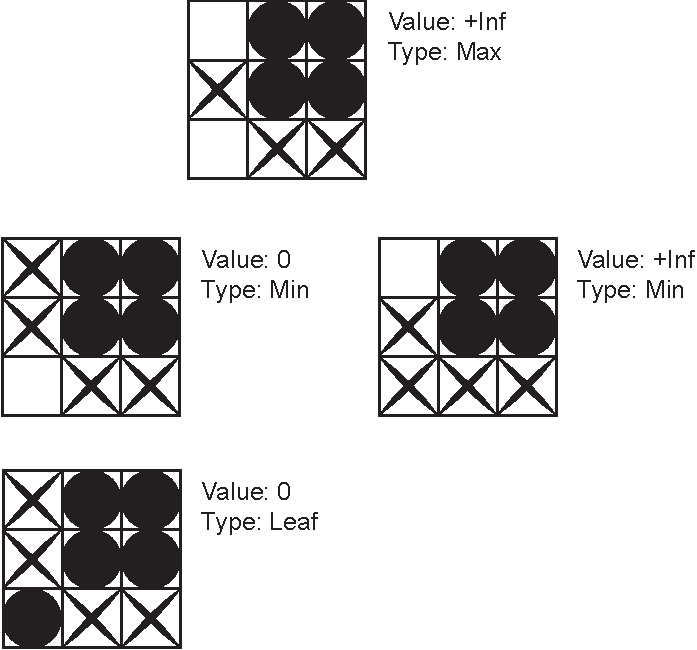
\includegraphics[width=0.6\textwidth]{minimax_tic_tac_toe.pdf}
\caption{Arbre Minimax per al jugador ``X'' en un moment donat del joc \emph{Tic-Tac-Toe}.}
\label{fig:minimax_tic_tac_toe}
\end{figure}

El problema de l'algorisme Minimax és que té un cost exponencial amb la profunditat de l'arbre, per això amb jocs amb molts torns o un gran nombre de moviments disponibles per torn, la seva profunditat màxima ha de limitar-se. A l'arribar a la profunditat màxima, per als nodes que no són finals, ha d'aplicar-se una funció heurística que determine el valor del node. L'elecció d'aquesta heurística és fonamental per a que la Intel·ligència Artificial que utilitza l'algorisme Minimax siga el millor possible, encara que l'arbre explorat no siga el complet.\\

L'algorisme \ref{alg:minimax} presenta el pseudocodi de l'algorisme Minimax sense restriccions de profunditat. La funció IsTerminal($s$) torna \emph{true} si l'estat $s$ és terminal o \emph{false} en cas contrari. La funció Type($s$) torna el tipus del node que representa l'estat $s$, els possibles valors són Max i Min. La funció Children($s$) genera una llista amb els nodes descendents de $s$ i finalment, la funció Movement($s$, $s'$) torna el moviment que s'ha de fer per passar de l'estat $s$ a l'estat $s'$. Quan un jugador inicia l'algorisme amb Minimax(EstatActual), obtindrà com a resposta el moviment que el conduirà a un millor resultat esperat.

\begin{algorithm}[H]
\caption{Minimax}
\label{alg:minimax}
\begin{algorithmic}[5]
\Require $s \in S$ to be a valid state of the game.
\Ensure $m$ is the best possible movement from state $s$, with an expected value of $v$. 
\If {IsTerminal(s)}
	\State \Return (Value(s), $\emptyset$)
\Else
	\If{ Type(s) = Max}
		\State $v \leftarrow -\infty$
		\State $m \leftarrow \emptyset$
		\ForAll{$s' \in $ Children($s$) }
			\State $v',m' \leftarrow$ Minimax($s'$)
			\If{$v' > v$}
				\State $v \leftarrow v'$
				\State $m \leftarrow$ Movement($s$, $s'$)
			\EndIf
		\EndFor
		\State \Return ($v, m$)
	\Else
		\State $v \leftarrow +\infty$
		\State $m \leftarrow \emptyset$
		\ForAll{$s' \in $ Children($s$) }
			\State $v',m' \leftarrow$ Minimax($s'$)
			\If{$v' < v$}
				\State $v \leftarrow v'$
				\State $m \leftarrow$ Movement($s$, $s'$)
			\EndIf
		\EndFor
		\State \Return ($v, m$)
	\EndIf
\EndIf
\end{algorithmic}
\end{algorithm}

Pot introduïr-se una component no-determinista per a escollir entre diversos moviments que tinguen un mateix valor. Basta amb avaluar els descendents d'un node de manera aleatòria (línies 7 i 18 de l'algorisme \ref{alg:minimax}). L'algorisme seguirà trobant el moviment òptim, però aquest no serà sempre el mateix en cas d'haver més d'un moviment òptim.\\

\subsection{Algorisme Negamax}
Per a aquells jocs on cada jugador no pot fer més d'un moviment successiu, existeix una simplificació de l'algorisme Minimax. L'algorisme Negamax\cite{knuth1976analysis} es basa en el fet que $\max(a,b) = -\min(-a,-b)$. D'aquesta manera no és necessari mantenir dos tipus de nodes distints en l'arbre i l'algorisme es simplifica considerablement. L'algorisme \ref{alg:negamax} descriu Negamax sense cap restricció sobre la profunditat.\\

\begin{algorithm}[H]
\caption{Negamax}
\label{alg:negamax}
\begin{algorithmic}[5]
\Require $s \in S$ to be a valid state of the game.
\Ensure $m$ is the best possible movement from state $s$, with an expected value of $v$. 
\If {IsTerminal(s)}
	\State \Return (Value(s), $\emptyset$)
\Else
	\State $v \leftarrow -\infty$
	\State $m \leftarrow \emptyset$
	\ForAll{$s' \in $ Children($s$) }
		\State $v',m' \leftarrow$ Negamax($s'$)
		\If{$-v' > v$}
			\State $v \leftarrow -v'$
			\State $m \leftarrow$ Movement($s$, $s'$)
		\EndIf
	\EndFor
	\State \Return ($v, m$)
\EndIf
\end{algorithmic}
\end{algorithm}

A l'igual que amb l'algorisme Minimax, pot introduir-se una component no-determinista si els descendents d'un node s'avaluen de manera aleatòria (línia 6 en l'algorisme \ref{alg:negamax}).\\

\subsection{Poda Alpha-Beta}
Existeix una tècnica per reduïr el nombre de nodes explorats en l'algorisme Minimax\cite{richards1961alpha} i que pot aplicar-se d'igual manera sobre l'algorisme Negamax\cite{knuth1976analysis}. La poda Alpha-Beta deu el seu nom a dos paràmetres $\alpha$ i $\beta$ que s'introdueixen sobre l'algorisme Minimax (o Negamax). \\

En un moment donat de l'execució de l'algorisme, el paràmetre $\alpha$ és el millor valor que pot aconseguir el jugador i proporciona una cota inferior al valor del node que s'està explorant. Per altra banda, $\beta$ és el millor valor que pot aconseguir l'oponent i proporciona una cota superior al valor del node. Cal observar que, si un node té un valor major que $\beta$, el predecessor d'aquest node, governat pel seu oponent, no elegirà el moviment que condueix al node actual, ja que té una altra alternativa que li garanteix un millor resultat, de manera que no és necessari seguir explorant el node actual.\\

L'algorisme \ref{alg:negamax_alphabeta} mostra el pseudocodi de l'algorisme Negamax amb la poda Alpha-Beta. El jugador que disposa del torn ha d'iniciar l'algorisme amb la crida NegamaxAB(EstatActual, $-\infty$, $+\infty$).

\begin{algorithm}[H]
\caption{Negamax with $\alpha-\beta$ prunning}
\label{alg:negamax_alphabeta}
\begin{algorithmic}[5]
\Require $s \in S$ to be a valid state of the game, $\alpha,\beta \in \mathbb{R}$.
\Ensure $m$ is the best possible movement from state $s$, with an expected value of $v$. 
\If {IsTerminal(s)}
	\State \Return (Value(s), $\emptyset$)
\Else
	\State $v \leftarrow \alpha$
	\State $m \leftarrow \emptyset$
	\ForAll{$s' \in $ Children($s$) $\wedge ~ v < \beta$}
		\State $v',m' \leftarrow$ NegamaxAB($s'$, $-\beta$, $-v$)
		\If{$-v' > v$}
			\State $v \leftarrow -v'$
			\State $m \leftarrow$ Movement($s$, $s'$)
		\EndIf
	\EndFor
	\State \Return ($v, m$)
\EndIf
\end{algorithmic}
\end{algorithm}

\subsection{Heurístiques}
Com s'ha comentat, no és possible explorar completament l'arbre Minimax o Negamax degut al cost exponencial que això suposa. Per tal d'evitar explorar l'arbre complet i obtenir una bona estimació del valor esperat i per tant, una bona estimació del millor moviment a elegir donat un estat, cal utilitzar una heurística que s'utilitzarà per a obtenir el valor dels nodes no terminals que es troben a una profunditat màxima determinada.\\

Les heurístiques depenen del joc en qüestió, a diferència dels algorismes Minimax i Negamax que són genèrics per a qualsevol tipus de joc de suma zero. A continuació es presenten dues heurístiques que s'han dissenyat per al joc del \emph{Connecta-4} i s'han implementat en el programa presentat.

\subsubsection{Heurística simple}\label{sec:heur_simple}
La primera heurística assigna el valor 0 a tots aquells nodes no terminals situats a la profunditat màxima. Aquesta heurística  pot considerar-se no-informada, ja que no utilitza la informació del node i dota a la Intel·ligència Artificial d'una estratègia molt poc sofisticada.

\begin{equation}
H_1(s) = \begin{cases}
+\infty & \text{IsTerminal}(s) \wedge \text{Winner}(s) = \text{RootPlayer}\\
- \infty & \text{IsTerminal}(s) \wedge \text{Winner}(s) \neq \text{RootPlayer}\\
0 & \text{otherwise}
\end{cases}
\end{equation}

\subsubsection{Heurística ponderada}\label{sec:heur_ponderada}
La segona heurística explora tots els possibles grups de quatre cel·les on un dels jugadors pot formar un \emph{Quatre en línia}. Llavors assigna un valor a cadascun d'aquests grups que depén dels discs que té cada jugador en el grup i el valor de la heurística és la suma dels valors de cada grup.\\

Es defineix un compador $C(g, p)$ que compta quants discs del jugador $p \in \{R, P\}$ ($R$ és el jugador de l'arrel de l'arbre i $P$ el seu oponent) hi han en el grup $g$. Llavors, el valor de l'heurística $H_G$ per al grup $g$ es defineix com:

\begin{equation}
H_G(g) = \begin{cases}
+\infty & C(g, R) = 4\\
-\infty & C(g, E) = 4\\
\lfloor \frac{C(g, R)}{3} \rfloor \cdot w_3 + &\\
\lfloor \frac{C(g, R)}{2} \rfloor \cdot w_2 + & \\
C(g, R) \cdot w_1&0 < C(g, R) \leq 3 \wedge C(g, E)  = 0\\
\lfloor \frac{C(g, E)}{3} \rfloor \cdot w_6 + &\\
\lfloor \frac{C(g, E)}{2} \rfloor \cdot w_5 + &\\
C(g, E) \cdot w_4 &C(G, R)  = 0 \wedge 0 < C(g, E) \leq 3\\
0 & \text{otherwise}
\end{cases}
\end{equation}

El valor de l'heurística per a l'estat $s$ ve determinat per l'equació següent:
\begin{equation}
H_2(s) = \sum_{g} H_G(g)
\end{equation}

L'heurística compta amb un vector de sis pesos $\mathbf{w} = w_1, \ldots, w_6$ que permet ajustar el seu comportament (d'ací sorgeix el nom de l'heurística). Cal observar que sols tenen sentit valors positius per als pesos $w_1$, $w_2$ i $w_3$, tenint en compte que el jugador arrel vol guanyar la partida, ja que aquests són considerats sols quan és aquest jugador qui té ventaja sobre el grup en qüestió. De la mateixa forma, sols tenen sentit valors negatius per als pesos $w_4$, $w_5$ i $w_6$, ja que en aquest cas és l'oponent qui té ventaja.\\

El nombre de grups de 4 cel·les que es poden formar en direccions horitzontal, vertical i les dues diagonals depèn de les dimensions del tauler, però en principi aquesta heurística no es troba restringida per les dimensions de cap tauler (sempre que el tauler en qüestió tinga almenys 4 columnes o 4 files).\\

La figura \ref{fig:connect4_example} mostra dos possibles estats del joc \emph{Connecta 4}. Suposant que el jugador a l'arrel és ``X'', el valor de l'heurística ponderada per al primer estat és $H_2(s_1) = 21 w_1 + 2 w_2 + 7 w_4 + 2 w_5 + w_6$. Pel que fa al segon estat, el valor de l'heurística és $H_2(s_2) = 12 w_1 + w_2 + 5 w_4$. Suposant que els pesos són $w_1 = 1, w_2 = 10, w_3 = 100, w_4 = -1, w_5 = -10$ i $w_6 = -100$, els valors finals de l'heurística per a ambdós estats són $H_2(s_1) = -76$ i $H_2(s_2) = 17$. Aquests valors són consistents amb la intuició de que l'estat $s_1$ és perjudicial per al jugador ``X'' ja que el jugador ``O'' pot guanyar amb un sol moviment a partir d'aquest estat.\\

\begin{figure}[h]
\centering
\begin{subfigure}[b]{0.4\textwidth}
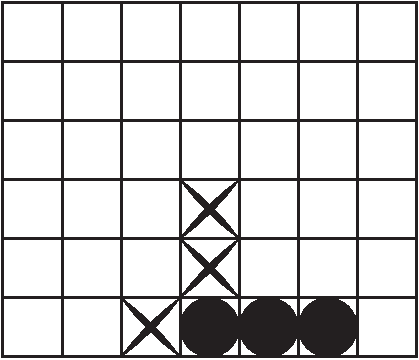
\includegraphics[width=\textwidth]{connect4_example.pdf}
\end{subfigure}
~
\begin{subfigure}[b]{0.4\textwidth}
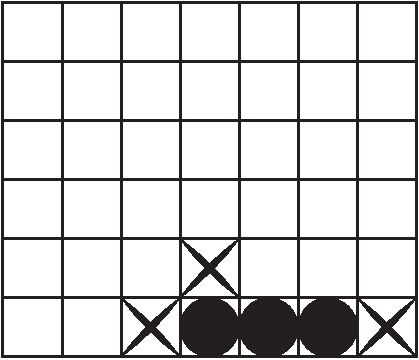
\includegraphics[width=\textwidth]{connect4_example2.pdf}
\end{subfigure}
\caption{Dos possibles estats per al joc \emph{Connecta 4}.}
\label{fig:connect4_example}
\end{figure}

\subsubsection{Selecció dels pesos de l'heurística ponderada}\label{sec:genetic}
L'elecció d'uns pesos adequats és fonamental per al bon funcionament d'aquesta heurística. Intuïtivament els pes dels grups de tres discs ha de ser major en valor absolut al pes dels grups de dos discs i aquest al pes dels grups d'una única peça. Inicialment i de manera intuïtiva, aquests pesos es van fixar segons la taula \ref{tab:init_weights}.\\

\begin{table}[h]
\centering
\begin{tabular}{|c|c|c|c|c|c|}
\hline $w_1$ & $w_2$  & $w_3$ & $w_4$ & $w_5$ & $w_6$ \\
\hline 1 & 5 & 100 & -2 & -10 & -200\\
\hline 
\end{tabular}
\caption{Pesos inicials fixats intuïtivament.}
\label{tab:init_weights}
\end{table}

El pesos $w_4$, $w_5$ i $w_6$ són majors en valor absolut als seus equivalents per al jugador arrel perquè s'intenta penalitzar aquells estats on els grups de cada jugador és similar, suposant que l'adversari sabrà aprofitar millor aquesta situació.\\

La intuició seguida a l'hora d'elegir els pesos de la taula \ref{tab:init_weights} no garantitza que aquests pesos siguen els òptims. Per tal de trobar aquests pesos òptims, en primer lloc, caldrà definir el criteri d'optimalitat per als pesos. Els pesos òptims seran aquells que, enfrontats amb tots els altres possibles pesos, són capaços de guanyar a la resta el major nombre de vegades. Per formalitzar aquesta idea, en primer lloc definim una funció que avalua el resultat d'un joc jugat utilitzant dos vectors de pesos. L'equació \ref{eq:Gdef} defineix aquesta funció, la qual anomenarem $G$.\\

\begin{equation}\label{eq:Gdef}
G(\mathbf{w^{(1)}}, \mathbf{w^{(2)}}) = \begin{cases}
+1 & \text{The winner is } \mathbf{w^{(1)}}\text{ when  } \mathbf{w^{(1)}} \text{ moves first}\\
-1 &\text{The winner is } \mathbf{w^{(2)}}\text{ when  } \mathbf{w^{(1)}} \text{ moves first}\\
0 & \text{Players draw when } \mathbf{w^{(1)}} \text{ moves first}
\end{cases}
\end{equation}

Si volem determinar quin dels dos pesos $\mathbf{w^{(1)}}$ i $\mathbf{w^{(2)}}$ és millor independentment de quin dels dos fa el primer moviment, basta amb utilitzar la mateixa funció però canviant l'ordre dels arguments i restant els valors. L'equació \ref{eq:player_comp} expressa aquesta idea.\\ 

\begin{equation}\label{eq:player_comp}
G(\mathbf{w^{(1)}}, \mathbf{w^{(2)}}) - G(\mathbf{w^{(2)}}, \mathbf{w^{(1)}}) = \begin{cases}
+2 & \mathbf{w^{(1)}} \text{ wins}\\
+1 & \mathbf{w^{(1)}} \text{ wins or draws}\\
0 & \text{Players draw} \\
-1 & \mathbf{w^{(1)}} \text{ loses or draws} \\
-2 & \mathbf{w^{(1)}} \text{ loses}
\end{cases}
\end{equation}

D'aquesta forma és senzill definir una funció de puntuació per a cadascun dels pesos (veure \ref{eq:weight_score}) i escollir aquells pesos emb el valor màxim en la seva funció de puntuació (equació \ref{eq:weight_opt}):\\

\begin{equation}\label{eq:weight_score}
S(\mathbf{w}) = \sum_{\mathbf{w'} \in \mathbb{R}^6} G(\mathbf{w}, \mathbf{w'}) - G(\mathbf{w'}, \mathbf{w})
\end{equation}

\begin{equation}\label{eq:weight_opt}
\mathbf{w^*} = \argmax_{\mathbf{w} \in \mathbb{R}^6} S(\mathbf{w})
\end{equation}

Cal observar que no necessàriament hi ha un únic òptim, ja que dos o més vectors de pesos poden vèncer sempre a resta de pesos i empatar quan s'enfronten entre ells. Però a més, aquest problema d'optimització és complex al ser el conjunt de pesos possibles infinit i al no ser derivable la funció a maximitzar, les tècniques d'optimització més emprades no són aplicables (ascens per gradient, gradient conjugat, etc). Per intentar relaxar el problema, definim una funció de puntuació alternativa que en lloc de comparar un vector de pesos amb la resta de possibles vectors, la compara amb un conjunt de pesos $B$ donat.\\

\begin{equation}\label{eq:weight_score_restricted}
S'(\mathbf{w}, B) = \sum_{\mathbf{w'} \in B \subseteq \mathbb{R}^6} G(\mathbf{w}, \mathbf{w'}) - G(\mathbf{w'}, \mathbf{w})
\end{equation}

Aquesta nova funció de puntuació dels pesos s'utilitza conjuntament amb un algorisme genètic per tal de trobar un bon vector de pesos. Per al funcionament d'aquest algorisme genètic primer es defineix una operació de \emph{Crossover} que combina dos vectors de pesos i una \emph{Mutation} que altera el valor d'un vector. L'operació de \emph{Crossover} (equació \ref{eq:crossover}) crea dos nous vectors de pesos intercanviant els elements de cada vector fins un punt de tall $p$. Aquest punt de tall es selecciona de manera uniforme entre els valors 1 i 5, de manera que es garanteix que els vectors produits no seran iguals als originals (a no ser que els vectors siguen iguals).\\

\begin{equation}\label{eq:crossover}
Crossover(\mathbf{w^{(1)}}, \mathbf{w^{(2)}}, p) =\begin{cases} 
(w^{(1)}_1,\ldots,w^{(1)}_p,w^{(2)}_{p+1},\ldots,w^{(2)}_{6})\\
(w^{(2)}_1,\ldots,w^{(2)}_p,w^{(1)}_{p+1},\ldots,w^{(1)}_{6})
\end{cases}
\end{equation}

L'operació \emph{Mutation} (equació \ref{eq:mutation}) inverteix el valor del bit $b$ de l'element $p$ d'un vector de pesos. Com que ens interessa que els elements 1,2 i 3 siguen valors positius i el 4, 5 i 6 siguen valors negatius, sols es modificarà la magnitud de l'element i no el seu signe. En l'equació \ref{eq:mutation} l'operador $\oplus$ fa referència a l'operador \emph{O-exlcussiva} i $\ll$ al desplaçament de bits a l'esquerra (cal observar que la implementació d'aquesta operació és depenent de la precisió utilitzada per a representar els elements del vector i la seva representació).\\

\begin{equation}\label{eq:mutation}
Mutation(\mathbf{w}, b, p) = (w_1, \ldots, w_{p-1}, w_p \oplus (1 \ll b), w_{p+1}, \ldots, w_6)
\end{equation}

L'algorisme \ref{alg:genetic_weights} defineix el procediment utilitzat per a escollir el vector de pesos final per a l'heurística ponderada. Com a paràmetres rep el nombre de generacions $G$, la grandària de la població $P$ i la grandària de els $N$-millors pesos a considerar per al còmput de la puntuació $S'$.\\

\begin{algorithm}
\caption{Genetic algorithm for choosing the best weights}
\label{alg:genetic_weights}
\begin{algorithmic}[5]
\Require $G, P, N \in \mathbb{N}, ~ P_{Crossover}, P_{Mutation} \in \mathbb{R}$
\State // Enumerable set of $P$ random weight vectors.
\State $W \leftarrow \{\mathbf{w^{(1)}}, \ldots, \mathbf{w^{(P)}} \}$ 
\State // Enumerable set of $N$ random weight vectors from $W$ ($B \subseteq W$).
\State $B \leftarrow \{\mathbf{b^{(1)}}, \ldots, \mathbf{b^{(N)}}\} \subseteq W$
\State // Evolve the population multiple generations.
\For{$g = 1$ \textbf{to} $G$}
    \State $W' \leftarrow \emptyset$
    \State // Mutate and cross individuals from the current generation.
	\For{$i = 1$ \textbf{to} $\lfloor \frac{W}{2} \rfloor$}
	    \State $\mathbf{u}, \mathbf{v} \leftarrow \mathbf{w^{(i)}}, \mathbf{w^{(\lfloor \frac{W}{2} \rfloor + i)}}$
	    \State Perform crossover between $\mathbf{u}$ and $\mathbf{v}$ with probability $P_{Crossover}$
	    \State Modify each bit of $\mathbf{u}$ and $\mathbf{v}$ with probability $P_{Mutation}$
	    		\State $W' \leftarrow W' \cup \{\mathbf{u}, \mathbf{v}\}$
	\EndFor
	\State // Choose the best individuals for the next generation.
	\State Compute the score $S'(\mathbf{w}, B), \forall \mathbf{w} \in W' \cup B$
	\State $W \leftarrow$ $P$-best weights in $W' \cup B$ according to $S'$
	\State $B \leftarrow$ $N$-best weights in $W$ according to $S'$
\EndFor
\State $\mathbf{b}^* \leftarrow$ Best weight in $B$ according to $S'$
\State \Return $\mathbf{b}^*$
\end{algorithmic}
\end{algorithm}

Cal observar que l'algorisme genètic és elitista ja que els millors individus de la generació $g$ també són candidats a formar part dels millors individus de la generació $g+1$. Cal observar que aquest algorisme no garantitza l'obtenció d'un òptim global, ni tan sols en el cas en que $N = P$, però com es comentarà en la secció d'experimentació obté uns resultats satisfactoris.\\

\section{Implementació}
La implementació del programa capaç de jugar al \emph{Connecta-4} s'ha fet en el llenguatge C++ intentant construïr una solució el més eficient possible en quant a requisits de memòria i processador. A més, el llenguatge C++ és un dels més estesos arreu del món i hi ha compiladors disponibles per a una gran varietat d'arquitectures de computadors i sistemes operatius. Les úniques biblioteques addicionals requerides són \emph{google-gflags}\footnote{\url{https://code.google.com/p/gflags/}} i \emph{google-glog}\footnote{\url{https://code.google.com/p/google-glog/}}, ambdues disponibles de manera gratuïta i llicenciades amb llicència BSD.\\

El programa compta amb distints mòduls que poden ampliar-se independentment per dotar al programa de més o millors funcionalitats. Les principals classes que poden extendre's per ampliar el programa són la classe \emph{Board} i \emph{Player}. La primera defineix el tauler del joc i la sèrie de moviments vàlids en un tauler i també defineix un mètode per avaluar el guanyador del joc. La classe Board implementa el joc clàssic de \emph{Connecta-4}, però pot ampliar-se per a permetre diverses modalitats del joc.\\

La classe  abstracta \emph{Player} representa el comportament d'un jugador. Hi ha distintes classes predefinides que implementen la classe \emph{Player}: \emph{HumanPlayer}, \emph{RandomPlayer}, \emph{NegamaxPlayer}, \emph{NegamaxAlphaBetaPlayer}, \emph{NetworkPlayer}, etc.\\

El codi font del projecte està disponible públicament\footnote{https://github.com/jpuigcerver/miarfid-atia-connect4} amb llicència GPLv3. A continuació s'expliquen els paràmetres dels dos principals programes.\\

\subsection{Programa \emph{weight\_tunning}}
El programa \emph{weight\_tunning} implementa l'algorisme genètic descrit en la secció \ref{sec:genetic} per tal d'obtenir un bon vector de pesos per a l'heurística ponderada. Aquest programa compta amb distintes opcions que governen el seu funcionament i que es mostren en la taula \ref{tab:weight_tunning_opts}.\\

\begin{table}[h]
\centering
\begin{tabular}{|l|c|l|}
\hline 
Opció & Valor per defecte & Descripció\\
\hline 
-crossover & 0.80 & Probabilitat de crossover entre dos individus\\
-generations & 1000 & Nombre de generacions\\
-mutation & 0.02 & Probabilitat de mutació d'un bit\\
-population & 1000 & Grandària de la població\\
-nbest & 5 & Nombre de millors vectors a considerar\\
-nthreads & 1 & Nombre de fils a utilitzar \\
-cols & 7 & Nombre de columnes del tauler\\
-rows & 6 & Nombre de files del tauler\\
-max\_depth & 5 & Profunditat màxima per a l'algorisme Negamax\\
-random & \emph{true} & Utilitza el Negamax no-determinista\\
-seed & 0 & Llavor per als nombres aleatoris\\
\hline
\end{tabular}
\caption{Opcions del programa \emph{weight\_tunning}}
\label{tab:weight_tunning_opts}
\end{table}

\subsection{Programa \emph{connect4}}
El programa \emph{connect4} implementa el joc en sí. Disposa de diferents opcions per controlar el seu comportament i que es mostren en la taula \ref{tab:connect4_opts}. El caràcter ``:'' separa els valors d'algunes opcions per a cada jugador (opcions -ai, -max\_depth, -random i -wh). \\

\begin{table}[h]
\centering
\begin{tabular}{|l|c|l|}
\hline 
Opció & Valor per defecte & Descripció\\
\hline 
-cols & 7 & Nombre de columnes del tauler\\
-rows & 6 & Nombre de files del tauler\\
-ai & \emph{Human}:\emph{Human} & Intel·ligència de cada jugador \\
-max\_depth & 5:5 & Profunditat màxima de Negamax\\
-o & - & Fitxer on es guarda la partida\\
-random & \emph{false}:\emph{false} & Utilitza el Negamax no-determinista\\
-seed & 0 & Llavor per als nombres aleatoris\\
\multirow{2}{*}{-wh} & 4;13;121;-10;-31;-128: & \multirow{2}{*}{Vector per a l'heurística ponderada}\\
& 4;13;121;-10;-31;-128 & \\
\hline
\end{tabular}
\caption{Opcions del programa \emph{connect4}}
\label{tab:connect4_opts}
\end{table}

Els distints tipus d'intel·ligències vàlides (opció -ai) són:
\begin{enumerate}
\item \emph{Human}: control per teclat
\item \emph{Random}: moviments aleatoris
\item \emph{SimpleNegamax}: heurística simple amb algorisme Negamax
\item \emph{SimpleAlphaBeta}: heurística simple amb algorisme Negamax i poda Alpha-Beta
\item \emph{WeightNegamax}: heurística ponderada amb algorisme Negamax
\item \emph{WeightAlphaBeta}: heurística ponderada amb algorisme Negamax i poda Alpha-Beta
\end{enumerate}

Els pesos de l'heurística s'indiquen utilitzant l'opció -wh. Si un dels dos jugadors no utilitza l'heurística ponderada, els valors del seu vector s'ignoren. Els distints elements de cada vector han d'anar separats amb un espai o un punt-i-coma (``;''). Els dos vectors, al igual que la resta d'opcions referents al jugador, van separats amb el caràcter dos-punts (``:'').

\section{Experiments}
\subsection{Selecció dels pesos de l'heurística ponderada}
Per a la selecció dels pesos de l'heurística ponderada (secció \ref{sec:heur_ponderada}) s'ha utilitzat l'algorisme genètic explicat en la secció \ref{sec:genetic} amb el paràmetres detallats en la taula \ref{tab:genetic_init}. Encara que l'algorisme \ref{alg:genetic_weights} no posa cap restricció sobre tipus de dades dels pesos, per a aquest experiment s'han considerat únicament pesos en el rang $[-128, 127]$ (valors enters amb signe de 8 bits). La duració de l'experiment en una màquina amb les especificacions de la taula \ref{tab:zoiberg} fou de 51 hores i 32 minuts. El vector de pesos obtingut finalment és el de la taula \ref{tab:best_weights}.\\

\begin{table}[h]
\centering
\begin{tabular}{|l|c|}
\hline 
Paràmetre & Valor \\
\hline
-crossover & 0.80\\
-mutation & 0.02\\
-population & 500\\
-cols & 7\\
-rows  & 6\\
-nbest & 5\\
-generations & 250\\
-max\_depth & 5 \\
-random & true\\
-nthreads & 4\\
-seed & 0\\
\hline
\end{tabular}
\caption{Paràmetres de l'algorisme genètic utilitzat per seleccionar els pesos de l'heurística ponderada.}
\label{tab:genetic_init}
\end{table}

\begin{table}[h]
\centering
\begin{tabular}{|l|l|}
\hline
Processador & Intel Core2 Duo, 2.33GHz\\
Memòria RAM & 2GB DDR2\\
Sistema Operatiu & Ubuntu 10.04 LTS (64 bits)\\
\hline
\end{tabular}
\caption{Característiques principals d'una de les màquines utilitzades per als experiments.}
\label{tab:zoiberg}
\end{table}

\begin{table}[h]
\centering
\begin{tabular}{|c|c|c|c|c|c|}
\hline $w_1$ & $w_2$  & $w_3$ & $w_4$ & $w_5$ & $w_6$ \\
\hline 4 & 13 & 121 & -10 & -31 &-128\\
\hline 
\end{tabular}
\caption{Vector de pesos escollit per l'algorisme genètic.}
\label{tab:best_weights}
\end{table}

\subsection{Comparativa dels resultats del joc}\label{sec:game_results}
El següent experiment permet obtenir quina és la millor heurística de les considerades:
\begin{enumerate}
\item \textbf{Aleatori}: Jugador que selecciona aleatòriament el moviment a fer entre la llista de moviments possibles.
\item \textbf{Simple}: Jugador que utilitza la cerca Negamax amb poda Alpha-Beta junt a l'heurística simple (secció \ref{sec:heur_simple}) per a elegir cada moviment.
\item \textbf{Heur.} $\mathbf{W_1}$: Jugador que utilitza la cerca Negamax amb poda Alpha-Beta i l'heurística ponderada (secció \ref{sec:heur_ponderada}) amb els pesos de la taula \ref{tab:init_weights}.
\item \textbf{Heur.} $\mathbf{W_2}$: Jugador que utilitza la cerca Negamax amb poda Alpha-Beta i l'heurística ponderada amb els pesos de la taula \ref{tab:best_weights}. Aquests pesos són el resultat de l'execució de l'algorisme genètic.
\end{enumerate}

Per als algorismes que utilitzen Negamax, s'ha limitat la seva profunditat a 5 nivells i s'ha utilitzat la cerca no-determinista. S'han fet 500 experiments distints per a cada parell de jugadors. La taula \ref{tab:expr_best_heur} resumeix els resultats obtinguts, indicant quin percentatge de vegades ha guanyat cada jugador ($R$ indica el percentatge de vegades que guanya el jugador fila, $C$ el jugador columna i $T$ el percentatge de vegades que han empatat). El jugador indicat en la fila és qui inicia el joc.\\

\begin{table}[h]
\centering
\begin{tabular}{|l|l|c|c|c|c|}
\hline
\multicolumn{2}{|c|}{} & Aleatori & Simple & Heur. $W_1$ & Heur. $W_2$\\
\hline
\multirow{3}{*}{Aleatori} & R & $56.0 \pm 4.4$ & $4.0 \pm 1.7$ & $4.0 \pm 1.6$  & $4.0 \pm 1.7$   \\
& C & $44.0 \pm 4.4$ & $96.0 \pm 1.7$ & $96.0 \pm 1.8$ & $96.0 \pm 1.7$\\
& T & $0.0 \pm 0.0$ & $0.0 \pm 0.0$ & $0.0 \pm 0.0$ & $0.0 \pm 0.0$ \\
\hline
\multirow{3}{*}{Simple} & R & $98.0 \pm 1.2$ & $52.0 \pm 4.4$ & $49.9 \pm 4.4$ & $52.0 \pm 4.4$\\
& C & $2.0 \pm 1.3$ & $41.0 \pm 4.3$ & $45.0 \pm 4.3$ & $44.0 \pm 4.3$\\
& T & $0.0 \pm 0.0$ & $7.0 \pm 2.2$ & $6.0 \pm 2.1$ & $5.0 \pm 1.8$\\
\hline
\multirow{3}{*}{Heur. $W_1$} & R & $100.0 \pm 0.0$ & $94.0 \pm 2.0$ & $32.0 \pm 4.1$ & $34.0 \pm 4.1$\\
& C & $0.0 \pm 0.0$ & $5.0 \pm 1.9$ & $68.0 \pm 4.1$ & $66.0 \pm 4.1$ \\
& T & $0.0 \pm 0.0$ & $1.0 \pm 1.0$ & $0.0 \pm 0.0$ & $0.0 \pm 0.0$ \\
\hline
\multirow{3}{*}{Heur. $W_2$} & R & $100.0 \pm 0.0$ & $97.0 \pm 1.8$ & $100.0 \pm 0.0$ & $100.0 \pm 0.0$ \\
& C & $0.0 \pm 0.0$ & $2.0 \pm 1.3$ & $0.0 \pm 0.0$ & $0.0 \pm 0.0$\\
& T & $0.0 \pm 0.0$ & $1.0 \pm 1.0$ & $0.0 \pm 0.0$ & $0.0 \pm 0.0$\\
\hline
\end{tabular}
\caption{Comparativa de victòries entre els distints jugadors. $R$ indica el percentatge de vegades que el jugador fila guanya, $C$ el jugador columna i $T$ les vegades que empaten. El jugador fila inicia el joc.}
\label{tab:expr_best_heur}
\end{table}

Si ens fixem en els casos en els que una heurística és enfrontada contra si mateixa (diagonal de la taula), observem que el jugador que inicia el joc té ventaja sobre el seu oponent, excepte en el cas de l'heurística $W_1$, en la que guanya en més ocasions el segon jugador. Aquest fet contradiu al que s'espera d'un jugador òptim, que deuria guanyar sempre que inicia el joc\cite{allis1988knowledge}.\\

No obstant això, l'heurística $W_2$ sí que es comporta com s'espera a l'enfrontar-se contra si mateixa. A més, aquesta heurística venç a la resta sempre que inicia el joc. Quan no l'inicia guanya també la major part de les partides, excepte a l'enfrontar-se contra l'heurística simple. En aquest cas, el percentatge de vegades que guanya $W_2$ és del $44\%$, front al $52\%$ que guanya l'heurística simple, però els intervals de confiança es solapen, de manera que no queda clar que iniciant el joc d'aquesta manera, l'heurística simple siga superior a l'heurística $W_2$.\\

En definitiva, l'algorisme genètic per seleccionar els pesos de l'heurística ponderada (algorisme \ref{alg:genetic_weights}) ha sigut capaç de seleccionar un vector de pesos millor que la resta d'heurístiques, incloent l'heurística $W_1$ construïda a partir de la intuició.

\subsection{Comparativa del nombre de nodes generats}
Per tal de comparar el nombre de nodes generats per l'algorisme Negamax s'han realitzat dos experiments. El primer té com a objectiu comparar l'algorisme Negamax i el Negamax amb poda Alpha-Beta. S'ha mesurat el nombre mitjà de nodes generats per a 500 partides enfrontant cada heurística contra si mateixa, amb la diferència de que un jugador utilitza l'algorisme Negamax sense poda i l'altre jugador amb poda Alpha-Beta. Els resultats d'aquest experiment es resumeixen en la taula \ref{tab:expr_nmax_ab}. La profunditat de l'arbre Negamax s'ha limitat igualment a 5 moviments i s'han utilitzat les versions no-deterministes dels algorismes.\\

\begin{table}[h]
\centering
\tabcolsep=0.09cm
\begin{tabular}{|l|l|c|c|}
\hline
\multicolumn{2}{|c|}{} & Full vs. $\alpha-\beta$ & $\alpha-\beta$ vs. Full \\
\hline
\multirow{2}{*}{Simple} & Full & $13249.77 \pm 1133.63$  & $13018.69 \pm 1114.28$ \\
& $\alpha-\beta$ & $601.05 \pm 52.40$ & $633.06 \pm 55.14$ \\
\hline
\multirow{2}{*}{Heur $W_1$} & Full & $12709.27 \pm 1083.02$ & $11978.66 \pm 1022.05$\\
& $\alpha-\beta$ & $1661.32 \pm 143.02$ & $1824.59 \pm 155.97$ \\
\hline
\multirow{2}{*}{Heur $W_2$} & Full & $12413.44 \pm 1047.38$  & $12420.26 \pm 1044.74$ \\
& $\alpha-\beta$ & $1864.43 \pm 157.20$ & $1820.21 \pm 153.94$\\
%Heur. $W_2$ & & & &\\
\hline
\end{tabular}
\caption{Nombre de nodes generats per moviment amb l'algorisme Negamax complet i amb poda Alpha-Beta. En cada columna canvia el jugador que inicia el joc. En cada fila, per a cada algorisme, el nombre de nodes generat utilitzant l'arbre complet i el podat.}
\label{tab:expr_nmax_ab}
\end{table}

S'observa en la taula \ref{tab:expr_nmax_ab} que el nombre de nodes generats utilitzant l'algorisme Negamax sense poda és al voltant d'un ordre de magnitud major que amb l'algorisme amb poda Alpha-Beta. No s'aprecien diferències significatives entre les dues heurístiques ponderades, utilitzant tant el Negamax amb poda com sense poda. Sí que s'observa que l'heurística simple amb poda Alpha-Beta genera molts menys nodes que la resta. La intuició inicial feia pensar que amb heurístiques més informades el nombre de nodes generats seria menor, però aquesta intuició és equivocada ja que una heurística no-informada pot realitzar podes que no beneficien al jugador i que no es farien amb més informació. La figura \ref{fig:comp_negamax_heur} mostra aquest fet en dos petits arbres Negamax. Els nodes no-terminals estan marcats amb un cercle i tenen els valors $(\alpha,\beta)$ inicials marcats a l'esquerra i els finals a la dreta. El valor de l'heurística per als nodes a profunditat màxima apareix en el centre del node. En aquest cas l'heurística no-informada generaria un node menys, però faria un moviment equivocat. La diferència de nodes generats pot accentuar-se a mesura que augmenten el nombre de moviments possibles en cada node i és el que explicaria el perquè l'heurística simple genera molts menys nodes que les heurístiques ponderades.\\

\begin{figure}[h]
\centering
\begin{subfigure}[b]{0.4\textwidth}
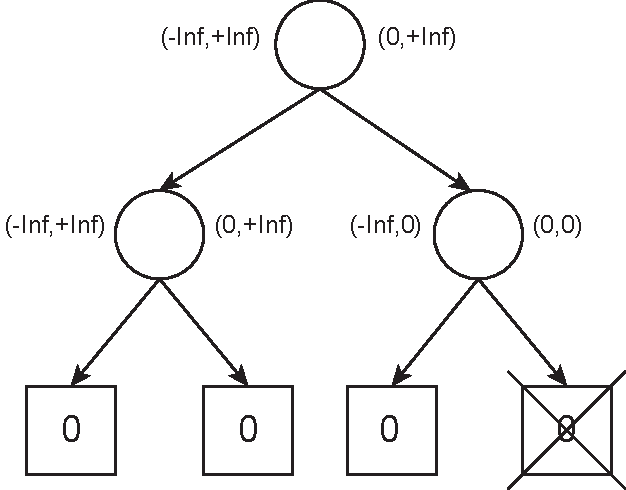
\includegraphics[width=\textwidth]{negamax_heur_simple.pdf}
\caption{Heurística no-informada}
\end{subfigure}
~
\begin{subfigure}[b]{0.4\textwidth}
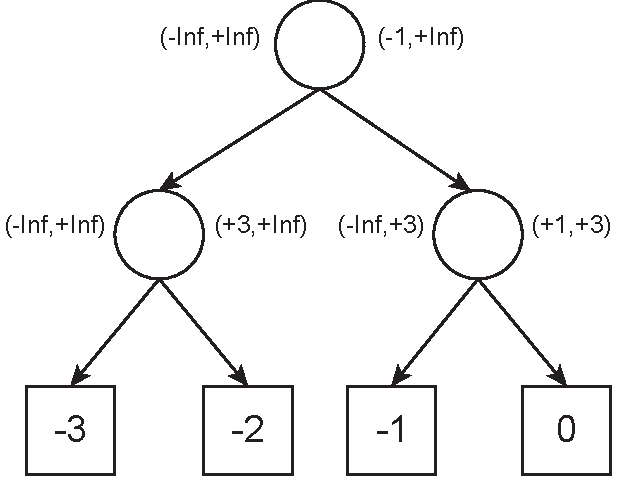
\includegraphics[width=\textwidth]{negamax_heur_informed.pdf}
\caption{Heurística informada}
\end{subfigure}
\caption{Arbres Negamax amb poda Alpha-Beta per a un mateix estat utilitzant dues heurístiques distintes: una no informada i l'altra informada.}
\label{fig:comp_negamax_heur}
\end{figure}

El segon experiment té la finalitat de comparar el nombre de nodes generats per l'algorisme Negamax amb poda Alpha-Beta quan l'oponent és una heurística diferent. S'han repetit els experiments de la secció \ref{sec:game_results} però ara mesurant el nombre mitjà de nodes generats per cada jugador en cada moviment.\\

\begin{table}[h]
\centering
\begin{tabular}{|l|l|c|c|c|}
\hline
\multicolumn{2}{|c|}{} & Simple & Heur. $W_1$ & Heur. $W_2$\\
\hline
\multirow{2}{*}{Simple} & $N_R$ & $626.87 \pm 54.55$ & $632.70 \pm 55.08$ & $640.78 \pm 55.70$\\
&  $N_C$ & $600.36 \pm 52.20$ & $599.89 \pm 52.29$ & $617.86 \pm 53.77$\\
\hline
\multirow{2}{*}{Heur. $W_1$} & $N_R$ & $1737.39 \pm 151.23$ & $1818.15 \pm 155.68$ & $1840.16 \pm 157.47$ \\
& $N_C$ & $581.98 \pm 50.17$ & $1655.80 \pm 142.56$ & $1664.04 \pm 143.28$ \\
\hline
\multirow{2}{*}{Heur. $W_2$} & $N_R$ & $1647.48 \pm 142.97$ & $1815.29 \pm 153.53$  &  $1841.40 \pm 155.73$ \\
& $N_C$ & $571.08 \pm 49.02$ & $1873.37 \pm 158.02$ & $1892.96 \pm 159.55$\\
\hline
\end{tabular}
\caption{Nombre de nodes generats per moviment entre els distints jugadors. $N_R$ indica el nombre mitjà de nodes del jugador fila i $N_C$ del jugador columna. El jugador fila inicia el joc.}
\label{tab:expr_nodes}
\end{table}

En la taula \ref{tab:expr_nodes} s'observa  de nou que l'heurística simple genera molts menys nodes que les heurístiques $W_1$ i $W_2$. Les heurístiques $W_1$ i $W_2$ generen un nombre similar de nodes. La mitjana de nodes generats per $W_2$ és generalment menor, però els intervals de confiança es solapen en totes les ocasions, de manera que les diferències no resulten significatives de manera estadística.\\

\section{Conclusions}
Com a resultat d'aquest treball s'ha implementat satisfactòriament el joc \emph{Connecta-4} per ordinador i s'ha dissenyat una heurística que, utilitzada junt a l'algorisme Negamax amb poda Alpha-Beta, és capaç de vèncer en el $99\%$ de les ocasions que inicia el joc i un $68.7\%$ de les vegades que no inicia el joc, comparat amb altres tres jugadors automàtics que equivaldrien a jugadors amb un distint grau de dificultat. Cal observar que l'estratègia òptima per al joc \emph{Connecta-4} garantitza un $100\%$ de les victòries quan s'inicia el joc\cite{allis1988knowledge}, de manera que l'heurística queda prop d'aquest objectiu. A més, s'ha dissenyat un algorisme genètic per a ajustar els paràmetres de l'heurística, aplicant no sols els coneixements d'Intel·ligència Artificial per a jocs de suma zero, sinó també coneixements sobre Algorismes Genètics.\\

Com a treball futur caldria comparar l'heurística ponderada amb l'estratègia òptima i veure com es comporta front aquesta. Un altre experiment que ha quedat pendent és el d'avaluar les distintes heurístiques amb diferents grandàries del tauler. Cal observar que el resultat de l'algorisme genètic de la secció \ref{sec:genetic} depèn de la grandària del tauler, així que és d'esperar que els pesos obtinguts no siguen els millors per a altres dimensions del tauler. D'altra banda, també seria interessant implementar una interfície gràfica per al programa i permetre jocs en xarxa, de manera que podrien fer-se competicions entre heurístiques dissenyades per diferents usuaris. Degut a la modularitat de la implementació, aquesta segona tasca és senzilla de fer i ja s'han iniciat els primers passos cap aquesta (pot consultar-se el jugador \emph{NetworkPlayer} en el codi font).

\bibliographystyle{ieeetr} 
\bibliography{report}

\end{document}